\appendix

\chapter{RAID 1}\label{anx:raid1}
    Consiste en una copia exacta de un conjunto de datos en dos o más discos. Resulta de utilidad cuando se busca seguridad a cambio de espacio de almacenamiento. Este tipo de configuraciones incrementa exponencialmente la fiabilidad respecto a un solo disco, es decir, la probabilidad de fallo del conjunto es igual al producto de las probabilidades de fallo de cada uno de los discos, ya que para que el conjunto falle es necesario que lo hagan todos sus discos. \cite{raid1-es} \cite{raid1-en}
    
    Además, \textit{RAID 1} presenta una mejora en las operaciones de lectura debido a que la información está presente en más de un disco y se puede acceder a múltiples datos de forma simultánea.

    \begin{figure}[h!]
    \centering
        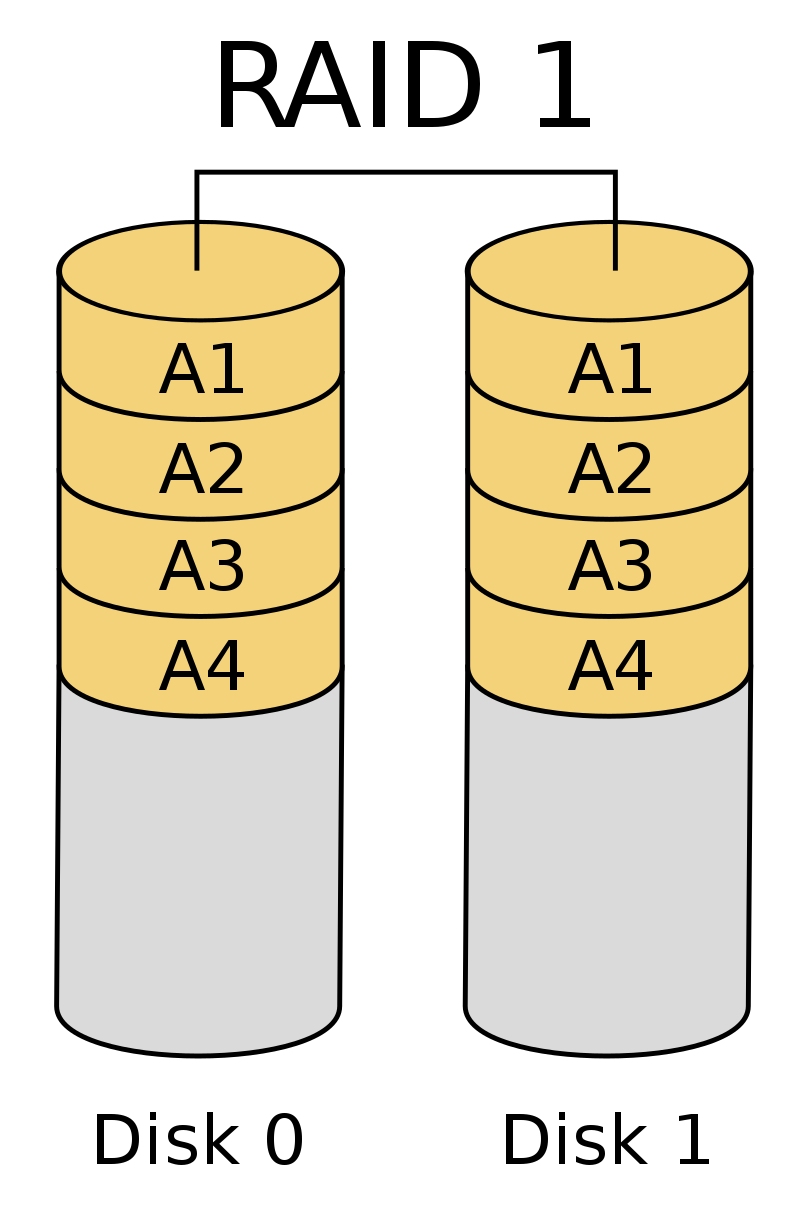
\includegraphics[scale=0.2]{raid1.png}
        \caption{Estructura RAID1}
        \label{fig:raid1}
    \end{figure}
    
    
\chapter{Filtro de errores}\label{anx:hw-info}
    \begin{figure}[H]
    \centering
        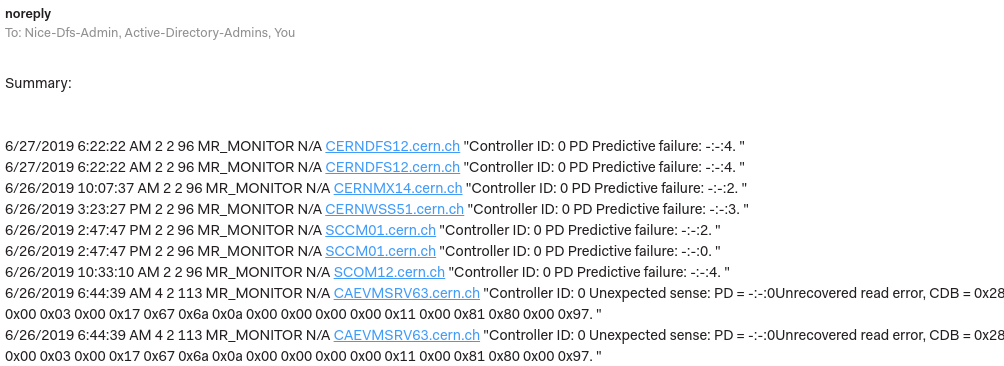
\includegraphics[scale=0.55]{filtro-de-errores.png}
        \caption{Filtro de errores de \textit{hardware}}
        \label{fig:error-filter}
    \end{figure}
    
    
\chapter{Listado de \textit{EventIDs} utilizados}\label{anx:eventid}
    \textbf{Winagent}
        \begin{enumerate}
            \setcounter{enumi}{-1}
            \item Error durante la administración del servicio
            \item Ha ocurrido un error general
            \item Error ejecutando el actualizador
            \item Se ha actualizado el sistema de actualización automática
            \item No hay \textit{plugins} que ejecutar
            \item Error al ejecutar un \textit{plugin}
            \item Archivo de configuración no encontrado.
            \item Error en el archivo de configuración
            \item Error obteniendo datos del archivo de configuración
            \item Archivos inválidos en la carpeta ``plugins''
            \item Error mientras se lanzaba un evento
            \item No se pudo encontrar el ejecutable del actualizador
            \item Ejecución de los \textit{plugins} superpuesta
        \end{enumerate}{}
        
        \textbf{Actualizador automático}
        \begin{enumerate}
            \setcounter{enumi}{-1}
            \item Error general del sistema
            \item Petición HTTP fallida
            \item Servicio no iniciado
            \item No se pudo guardar un archivo
            \item No se pudo encontrar el directorio ``tmp''
            \item No se pudo encontrar la ruta al archivo de configuración
            \item Error en el archivo de configuración
            \item Error obteniendo datos del archivo de configuración
            \item Componente actualizada
        \end{enumerate}{}
        
    
\chapter{Ejemplo de configuración real}\label{anx:settings}
    \begin{lstlisting}[style=csharp, caption=Fichero de configuración]
        {
          "autoUpdates": {
            "enabled": true,
            "source": "gitlab",
            "uri": "https://gitlab.cern.ch/api/v4/projects/winagent%2F{plugin}/releases/production",
            "schedule": {
              "seconds": 0,
              "minutes": 5,
              "hours": 1
            }
          },
          "eventLogs": [
            {
              "name": "Application",
              "outputPlugins": [
                {
                  "name": "RabbitMQ",
                  "settings": {
                    "servers": [
                      {
                        "hostName": "restricted.cern.ch",
                        "userName": "restricted",
                        "password": "restricted",
                        "queueName": "logs",
                        "virtualHost": "test"
                      },
                      {
                        "hostName": "restricted.cern.ch",
                        "userName": "restricted",
                        "password": "restricted",
                        "queueName": "logs",
                        "virtualHost": "test"
                      }
                    ]
                  }
                }
              ]
            },
            {
              "name": "System",
              "outputPlugins": [
                {
                  "name": "RabbitMQ",
                  "settings": {
                    "servers": [
                      {
                        "hostName": "restricted.cern.ch",
                        "userName": "restricted",
                        "password": "restricted",
                        "queueName": "logs",
                        "virtualHost": "test"
                      },
                      {
                        "hostName": "restricted.cern.ch",
                        "userName": "restricted",
                        "password": "restricted",
                        "queueName": "logs",
                        "virtualHost": "test"
                      }
                    ]
                  }
                }
              ]
            }
          ],
          "inputPlugins": [
            {
              "name": "Storcli",
              "settings": {
              },
              "outputPlugins": [
                {
                  "name": "RabbitMQ",
                  "settings": {
                    "servers": [
                      {
                        "hostName": "restricted.cern.ch",
                        "userName": "restricted",
                        "password": "restricted",
                        "queueName": "Storcli",
                        "virtualHost": "test"
                      },
                      {
                        "hostName": "chopin-amqp-d.cern.ch",
                        "userName": "restricted",
                        "password": "restricted",
                        "queueName": "Storcli",
                        "virtualHost": "test"
                      }
                    ]
                  },
                  "schedule": {
                    "seconds": 0,
                    "minutes": 2,
                    "hours": 0
                  }
                }
              ]
            },
            {
              "name": "Facter",
              "settings": {
              },
              "outputPlugins": [
                {
                  "name": "RabbitMQ",
                  "settings": {
                    "servers": [
                      {
                        "hostName": "restricted.cern.ch",
                        "userName": "restricted",
                        "password": "restricted",
                        "queueName": "Facter",
                        "virtualHost": "test"
                      },
                      {
                        "hostName": "restricted.cern.ch",
                        "userName": "restricted",
                        "password": "restricted",
                        "queueName": "Facter",
                        "virtualHost": "test"
                      }
                    ]
                  },
                  "schedule": {
                    "seconds": 0,
                    "minutes": 2,
                    "hours": 0
                  }
                }
              ]
            },
            {
              "name": "Updates",
              "settings": {
              },
              "outputPlugins": [
                {
                  "name": "RabbitMQ",
                  "settings": {
                    "servers": [
                      {
                        "hostName": "restricted.cern.ch",
                        "userName": "restricted",
                        "password": "restricted",
                        "queueName": "Updates",
                        "virtualHost": "test"
                      },
                      {
                        "hostName": "restricted.cern.ch",
                        "userName": "restricted",
                        "password": "restricted",
                        "queueName": "Updates",
                        "virtualHost": "test"
                      }
                    ]
                  },
                  "schedule": {
                    "seconds": 0,
                    "minutes": 0,
                    "hours": 1
                  }
                }
              ]
            },
            {
              "name": "Heartbeat",
              "settings": {
              },
              "outputPlugins": [
                {
                  "name": "RabbitMQ",
                  "settings": {
                    "servers": [
                      {
                        "hostName": "restricted.cern.ch",
                        "userName": "restricted",
                        "password": "restricted",
                        "queueName": "Heartbeat",
                        "virtualHost": "test"
                      },
                      {
                        "hostName": "restricted.cern.ch",
                        "userName": "restricted",
                        "password": "restricted",
                        "queueName": "Heartbeat",
                        "virtualHost": "test"
                      }
                    ]
                  },
                  "schedule": {
                    "seconds": 0,
                    "minutes": 2,
                    "hours": 0
                  }
                }
              ]
            },
            {
              "name": "Superdoctor",
              "settings": {
              },
              "outputPlugins": [
                {
                  "name": "RabbitMQ",
                  "settings": {
                    "servers": [
                      {
                        "hostName": "restricted.cern.ch",
                        "userName": "restricted",
                        "password": "restricted",
                        "queueName": "Superdoctor",
                        "virtualHost": "test"
                      },
                      {
                        "hostName": "restricted.cern.ch",
                        "userName": "restricted",
                        "password": "restricted",
                        "queueName": "Superdoctor",
                        "virtualHost": "test"
                      }
                    ]
                  },
                  "schedule": {
                    "seconds": 0,
                    "minutes": 0,
                    "hours": 1
                  }
                }
              ]
            }
          ]
        }
    \end{lstlisting}